\subsection{Worksheet - Double Pendulum}
\begin{center}
    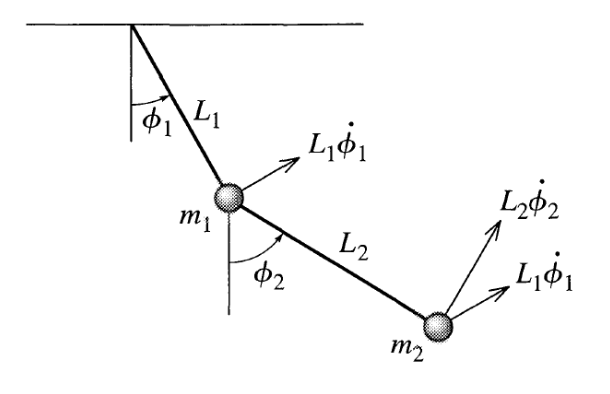
\includegraphics[scale=0.5]{Lecture-11/w11-img1.png}
\end{center}
\begin{p}
Find the potential energy of the double pendulum.
\end{p}
\begin{s}
The height of the first mass is given by $L_1(1-\cos\phi_1)$, and the height of the second mass is given by $L_1(1-\cos\phi_1) + L_2(1-\cos\phi_2)$ by trigonometry (the second mass is just the height of the first + the relative height from the first mass). Hence the total potential energy is given by:
\[U = U_1 + U_2 = m_1gL_1(1-\cos\phi_1) + m_2gL_1(1-\cos\phi_1) + m_2gL_2(1-\cos\phi_2)\]
\end{s}

\begin{p}
Write the kinetic energy in terms of $\dot{\phi}^2_1$ and $\dot{\phi}^2_2$
\end{p}
\begin{s}
The first mass is easy; it is just $T_1 = \frac{1}{2}m_1L^2\dot{\phi}_1^2$. The second term is slightly harder as the position vector is given by the sum of the vector from the fixed point to $m_1$ plus the vector from $m_1$ to $m_1$. Expanding this out, this yields total kinetic energy:
\[T = \frac{m_1}{2}L_1\dot{\phi}_1^2 + \frac{m_2}{2}\left(L_1^2\dot{\phi}_1^2 + L_2^2\dot{\phi}_2^2 + 2L_1L_2\dot{\phi}_1\dot{\phi}_2\cos(\phi_1 - \phi_2)\right)\]
Note the cross term we get at the end.
\end{s}

\begin{p}
Write the kinetic and potential energies in the simplifying case where the angles $\phi_i$ and their derivatives $\dot{\phi}_i$ are small.Find the two equations of motion in this case. 
\end{p}
\begin{s}
Time for the small angle approximation! In the limit of small angles, $\cos\phi \approx 1 - \frac{\phi^2}{2}$ and so the potential energy reduces to:
\[U = \frac{m_1 + m_2}gL_1\phi_1^2 + \frac{m_2}{2}gL_2\phi^2_2\]
For the kinetic term, the only cosine that shows up is the last term. We do have to be slightly careful here as expanding this out, we already get terms that are nonlinear (e.g. $(\phi_1 - \phi_2)^2$). We only want terms of order 2 and lower in our expression, (e.g. $\phi^2, \phi\dot{\phi}, \dot{\phi}^2$) so in our expansion of $\cos(\phi_1 - \phi_2)$ we only keep the highest order term (e.g. just $1$)! Thus the kinetic energy reduces to:
\[T = \frac{m_1 + m_2}{2}L_1^2\dot{\phi}_1^2 + m_2L_1L_2\dot{\phi}_1\dot{\phi}_2 + \frac{m_2}{2}L_2^2\dot{\phi}_2^2\]
\end{s}

\begin{p}
From the two linearized equations of motion for the double pendulum, find the corresponding matrices $\MM$ and $\KK$.
\end{p}
\begin{s}
The EL equations yield:
\[(m_1 + m_2)L_1^2\ddot{\phi}_1 + m_2L_1L_2\ddot{\phi}_2 = -(m_1 + m_2)gL_1\phi_1\]
\[m_2L_1L_2\ddot{\phi}_1 + m_2L_2^2\ddot{\phi}_2 = -m_2gL_2\phi_2\]
Which we can see are (fortunately) linear from our small angle simplification above. We can write these equations in matrix form:
\[\MM\ddot{\bm{\phi}} = -\KK\bm{\phi}\]
Writing out these matrices, we have:
\[\MM = \m{
(m_1 + m_2)L_1^2 & m_2L_1L_2
\\ m_2L_1L_2 & m_2L_2^2}\]
\[\KK = \m{(m_1 + m_2)gL_1 & 0 
\\ 0 & m_2gL_2}\]

\end{s}

\begin{p}
What are the eigenfrequencies and eigenvectors (the normal modes) when $m_1 = m_2 = m$ and $l_1 = l_2 = l$?
\end{p}
\begin{s}
In the case that all the masses and lengths are the same, we may write these matrices as:
\[\MM = mL^2\m{2 & 1 \\ 1 & 1}\]
\[\KK = mL^2\m{2\omega_0^2 & 0 \\ 0 & \omega_0^2}\]
Where we introduce $\omega_0 = \sqrt{\frac{g}{l}}$. Exactly as we did last day, we make an Ansatz:
\[\v{z} = \v{a}\exp(i\omega t)\]
This generates a characteristic equation for the eigenvalues:
\[\det(\KK - \omega^2\MM) = 0\]
Expanding this out, we have:
\[\det(mL^2\m{2(\omega_0^2 -\omega^2) & -\omega^2 \\ -\omega^2 & (\omega_0^2 - \omega^2)}) = 0\]
Which yields the equation:
\[2(\omega_0^2 - \omega^2)^2 - \omega^4 = \omega^4 - 4\omega_0^2\omega^2 + 2\omega_0^4 = 0\]
This is a quadratic equation in $\omega^2$, which has roots:
\[\omega_{1/2}^2 = 2\omega_0^2 \pm\sqrt{\frac{16\omega_0^2 - 8\omega_0^2}{4}} = \omega_0^2\left(2\pm \sqrt{2}\right)\]
Now solving for the normal modes (e.g. the eigenvectors), we get solutions:
\[\phi_I(t) = A\m{1 \\ \sqrt{2}}\cos(\omega_1 t - \delta)\]
\[\phi_II(t) = A\m{1 \\ -\sqrt{2}}\cos(\omega_2 t - \delta)\]
We see that this is similar to the results of last day (one mode with the two masses in phase, one mode with the two masses out of phase), but with a difference that the lower mass has a greater amplitude.
\newline\textit{Remark:} After linearization, the problem solving method reduces to what we saw last day; without linearization, the double pendulum system is chaotic! Perhaps to be revisited at the end of this class. But for small deviations from local minima in the potential, this method is generally feasible.
\end{s}